% v2-acmtog-sample.tex, dated March 7 2012
% This is a sample file for ACM Transactions on Graphics
%
% Compilation using 'acmtog.cls' - version 1.2 (March 2012), Aptara Inc.
% (c) 2010 Association for Computing Machinery (ACM)
%
% Questions/Suggestions/Feedback should be addressed to => "acmtexsupport@aptaracorp.com".
% Users can also go through the FAQs available on the journal's submission webpage.
%
% Steps to compile: latex, bibtex, latex latex
%
% For tracking purposes => this is v1.2 - March 2012
\documentclass{acmtog} % V1.2

%\acmVolume{VV}
%\acmNumber{N}
%\acmYear{YYYY}
%\acmMonth{Month}
%\acmArticleNum{XXX}
%\acmdoi{10.1145/XXXXXXX.YYYYYYY}
\acmVolume{28}
\acmNumber{4}
\acmYear{2019}
\acmMonth{September}
\acmArticleNum{106}
\acmdoi{10.1145/1559755.1559763}

\usepackage[namelimits]{amsmath} %数学公式
\usepackage{amssymb}             %数学公式
\usepackage{amsfonts}            %数学字体
\usepackage{mathrsfs}            %数学花体
\usepackage[options ]{algorithm2e}
\usepackage[colorlinks,
            linkcolor=blue,       %%修改此处为你想要的颜色
            anchorcolor=blue,  %%修改此处为你想要的颜色
            citecolor=blue,        %%修改此处为你想要的颜色,例如修改blue为red
            ]{hyperref}

\begin{document}

\markboth{GAN+RL For Anoamly Detection}{GAN+RL For Anomaly Detection}

\title{GAN+RL For Anomaly Detection} % title

\author{Quanyu Long {\upshape and} Haoxuan Wang
\affil{Shanghai Jiao Tong University}
\affil{516030910551 \quad 516030910514}
\affil{oscar.long@sjtu.edu.cn \quad hatchet25@sjtu.edu.cn}
% NOTE! Affiliations placed here should be for the institution where the
%       BULK of the research was done. If the author has gone to a new
%       institution, before publication, the (above) affiliation should NOT be changed.
%       The authors 'current' address may be given in the "Author's addresses:" block (below).
%       So for example, Mr. Fogarty, the bulk of the research was done at UIUC, and he is
%       currently affiliated with NASA.
}


\maketitle

\section{Introduction}
With the development of computing technology and Internet technology, computer networks are becoming increasingly important. Massive infrastructures based on these networks have significant impact on modern society. However, with the expanding size of complex networks, it becomes gradually harder for people to maintain the safety of these systems. Thus, anomaly detection done by computer programs is essential as it cost too much for people to identify the anomalies by naked eyes. In this paper, we aim to detect the anomalies that occur in web servers. 

Detection of web traffic anomalies in web servers is a univariate time-series classification problem. However, this classification problem is different from classical ones because the abnormal samples occur rarely, that is, they only take up a very small part of the total samples. Thus, traditional classification methods does not perform well on this problem as the models could only learn the features from normal samples, but does not have the ability to discriminate between normal and abnormal ones. 

There are three kinds of anomaly type: contextual anomaly, point anomaly and collective anomaly, which are results of different web attacks. These anomalies may contain both local and global patterns, where global ones are easier to identify but the local ones having the same distribution as normal data and therefore harder to detect. This makes the question harder, and common deep learning models are not qualified to solve this problem.  

In this paper, we firstly design a deep learning model(CLSTM) for anomaly detection, pre-processing data wisely to avoid data imbalance. Then a new model combining CLSTM, GAN, and reinforcement learning to detect anomalies in the dataset.

\section{Background}
Many researchers have studied the classification of normal and abnormal patterns by extracting the data features in the field of anomaly detection. Traditional methods such as K-means (calculating the distance between centroids and feature value), random forest (an unsupervised learning method that can extract outlier patterns) and SVM (using different kernels) are used and have achieved great performance at classifying statistical anomalies, but they cannot properly classify abnormal data that has the same distribution as the normal data. 

As deep learning networks are developed, we are motivated to use them to extract the hidden features of data. RNN networks such as LSTM were used to predict future signals and then calculate error distributions. These methods are good at dealing with data that as periodicity and can achieve high classification performance. But with data that do not have periodicity, the performance decrease greatly. CNN could also be used. Sequential data could be mapped into a multi-dimensional image and passed through the neural network to extract its spatial features. However, when we are dealing with time series data, time information is lost in the convolution and pooling operations. Thus, constructing a model that can both extract temporal and spacial features in data sequences is of vital importance. C-LSTM(proposed by Chunting Zhou, Chonglin Sun, 2015\cite{bibitem6}) is to make use of the two features. It consists of CNN and LSTM layers, structured linearly. The spatial features of the data sequence is extracted by the convolution and pooling layers, and the temporal features are extracted by the LSTM layers. C-LSTM was proposed to do text classification, we redesigned the network structure and use it to do anomaly detection.

But a more innovative idea came out when GAN was inspected in the field anomaly detection. Since GAN is able to able to generate data of a particular distribution, we are motivated to use GAN to generate the value distribution of normal data, and since normal and abnormal data have different distributions, we are able to classify them. The classification, also called anomaly assessment, is to calculate the distance between test data and the normal distribution. When the distance is too far(over some limit), we can label that data as abnormal. Work of this was first done by Houssam Zenati and Chuan-Sheng Foo in 2018\cite{bibitem1}. They took a DNN as a generator and another DNN as the discrimminator, and assessed the anomalies by transforming the test data and generated data into latent space to calculate their distance. State-of-art performance was obtained by their model. However, their work only dealt with data that does not possess temporal features, and does not perform well on data with time series. GAN models that deal with time series also exist, and the most well-known one is SeqGAN, which generates word sentences. It contains LSTM to extract the word sequence time features. However, the data for this method is discrete, we are able to construct a dictionary to store all the words, but anomaly detection does not have a notion of dictionary since some features are continuous. Thus, SeqGAN cannot be used for anomaly detection directly, but we can adopt some of its ideas, such as reinforcement learning, in our model.

As described above, there are many methods to perform anomaly detection on data sequences. C-LSTM did well in extracting temporal-spatial features, while GAN is good at learning the value distribution of the data. Therefore, we came up with the idea to combine these features together by constructing a model using CNN, RNN, GAN and reinforcement learning.


\section{Our Model}
Our model combines CNN and LSTM as classifier,which already get high performance on on Yahoo’s well-known Webscope S5 dataset. In addition, to solve the imbalanced data problem, we proposed a network combining GAN and reinforcement learning. This section will firstly introduce the deep learning model, inspiration of GAN with RL, and our algorithm.

\subsection{C-LSTM Classifier for AD}

\begin{figure*}
	\begin{center}
		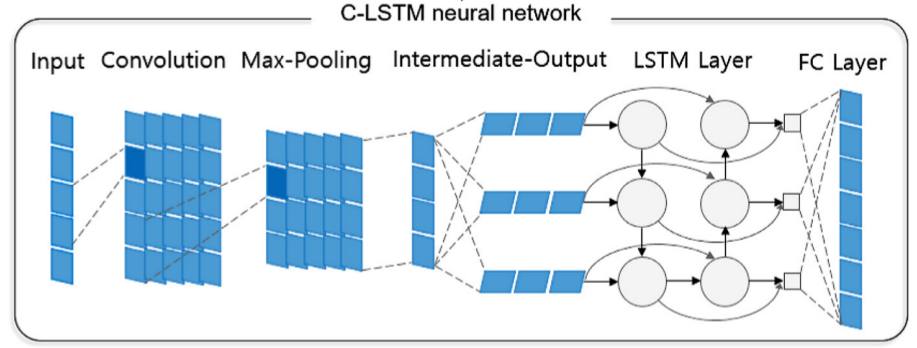
\includegraphics[width=0.9\textwidth]{C-LSTM.png}
	\end{center}
	\caption{C-LSTM Structure}
	\label{RTL}
\end{figure*}

The proposed deep learning model consists of CNN and LSTM layers, and is connected in a linear structure. Figure 1 represents the structure for anomaly detection of web traffic using the proposed C-LSTM. The C-LSTM uses the preprocessed data as inputs. Input is a sequence of data consisting of time serial normal and abnormal web traffic data, once a sequence has an abnormal data, then the sequence is abnormal. The spatial features in the traffic window are extracted by the LSTM layers. The temporal features are then extracted by the LSTM layers. The trained model then performs anomaly detection on the test data using a softmax classifier.

We designed the parameters of C-LSTM as listed in Table 1. The input of the C-LSTM is a data vector of length 60 that passes through the LSTM after passing through the convolution and pooling layers. We used tanh as an activation function of C-LSTM. Tanh is a function that rescales and shifts the sigmoid function, so that tanh is faster in learning than sigmoid when it is used as an activation function. There is an- other activation function like ReLU other than tanh. ReLU computes the function $f(x)=max⁡(0,x)$. In other words, it thresholds the activation at zero. Its advantage is that it greatly accelerates the convergence of the stochastic gradient descent compared to the tanh function, which is claimed to be due to its linear form. Also, when compared to a tanh neuron containing expensive operations, ReLU can be computed with a simple operation. Although the proposed architecture uses tanh, there could be improvements with ReLU or its relatives.

The proposed C-LSTM method outperforms other state-of-the-art machine learning techniques.

\begin{table}[h]
\tbl{Parameters for Sliding Window}{
\begin{tabular}{|l|l|c|c|}
	\hline
	Type & Filter & Kernel size & Stride     \\ 
	\hline
	Convolution & 64 & 5 & 1 \\
	Activation(tanh) & - & - &- \\
	Pooling & - & 2 & 2 \\
	Convolution & 64 & 5 & 1 \\
	Activation(tanh) & - & - &- \\
	Pooling & - & 2 & 2 \\
	LSTM(64) & - &- & - \\
	Dense(32) & - &- & - \\
	Activation(tanh) & - & - &- \\
	Dense(2) & - &- & - \\
	Softmax & - & - & - \\
	\hline
\end{tabular}}
\end{table}

\subsection{GAN for AD}
Till now, we design a deep learning network for classification. However, when our training set contains little positive samples (abnormal samples), the deep learning training procedure cannot ensure the model to learn how to classify the normal and abnormal, that is the data imbalanced problem.

The initial purpose to apply GAN on anomaly detection task is to learn the distribution of normal status, then through the discrepancy between the real samples and learned distribution, we can judge whether the testing sample is in anomalous status.

Related works of GAN for AD just apply the traditional neural network in generator and discriminator, not using the spatial and temporal information, which motivate us to propose a sequence GAN network. In addition, to avoid discrete data problem in GAN, we combine the GAN and reinforcement learning.

\subsection{GAN via Policy Gradient}
When noise passes through deep neural network, we gain the generated data, and we call the generated data as action. When passing the generated data to the C-LSTM classifier which we introduce before, we can get a score, which represents the policy, we denote as $G_{\theta}(y|s_{0} )$, $s_{0}$ is the state of the hidden layers in LSTM. To apply policy gradient, we still need an action-value function of generated data, we denote as $Q_{D_{\phi}}^{G_{\theta}}(a,s_{0})$. This function takes the action and the states, and output a reward, here we consider the estimated probability of being real by the discriminator $D_{\phi}(h_{1:T})$ as reward. We have:

\begin{equation}
Q_{D_\phi}^{G_\theta}(a = y, s = h_{1:T}) = D_\phi(h_{1:T})
\label{eq:samplevar}
\end{equation}

A benefit of using the discriminator as a reward function is that it can be dynamically updated to further improve the generative model iteratively. The network of discriminator is shown in Figure 2, which outputs the logits $D_{\phi}(h_{1:T})$, that is reward. Noting that there are multiple intermediate layers, these layers are designed to help to do anomaly assessment, which will be discussed in 3.5.

\begin{figure*}
   \begin{center}
      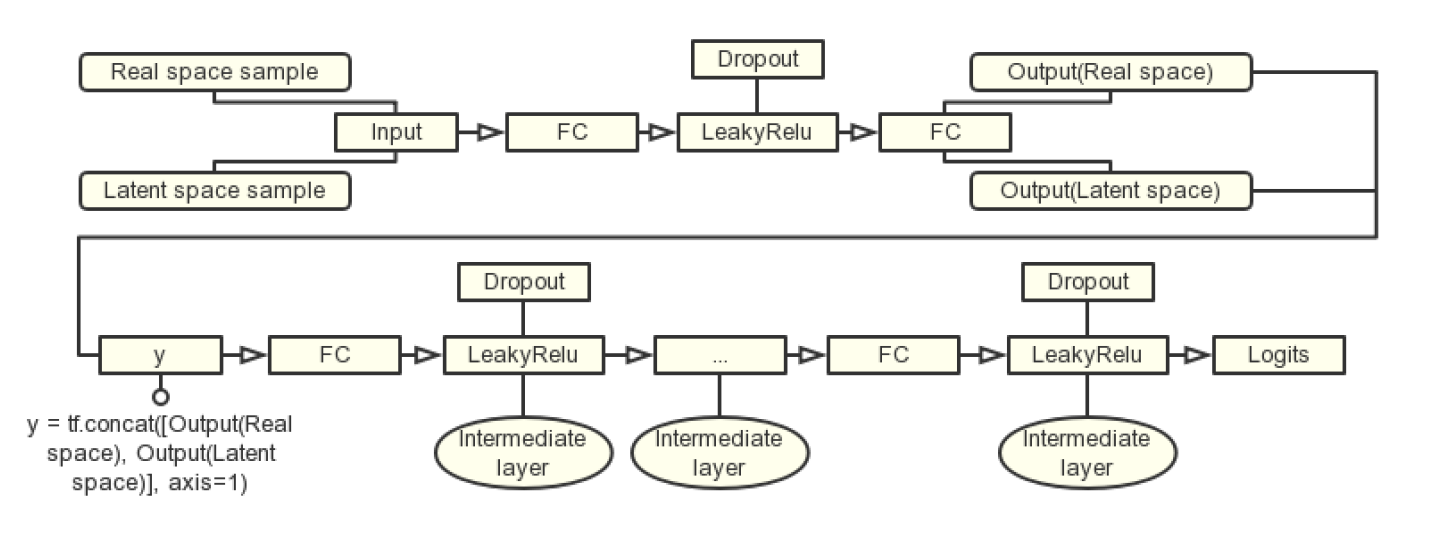
\includegraphics[width=0.9\textwidth]{dis.png}
   \end{center}
\caption{The discriminator network}
\label{RTL}
\end{figure*}

\begin{figure*}
	\begin{center}
		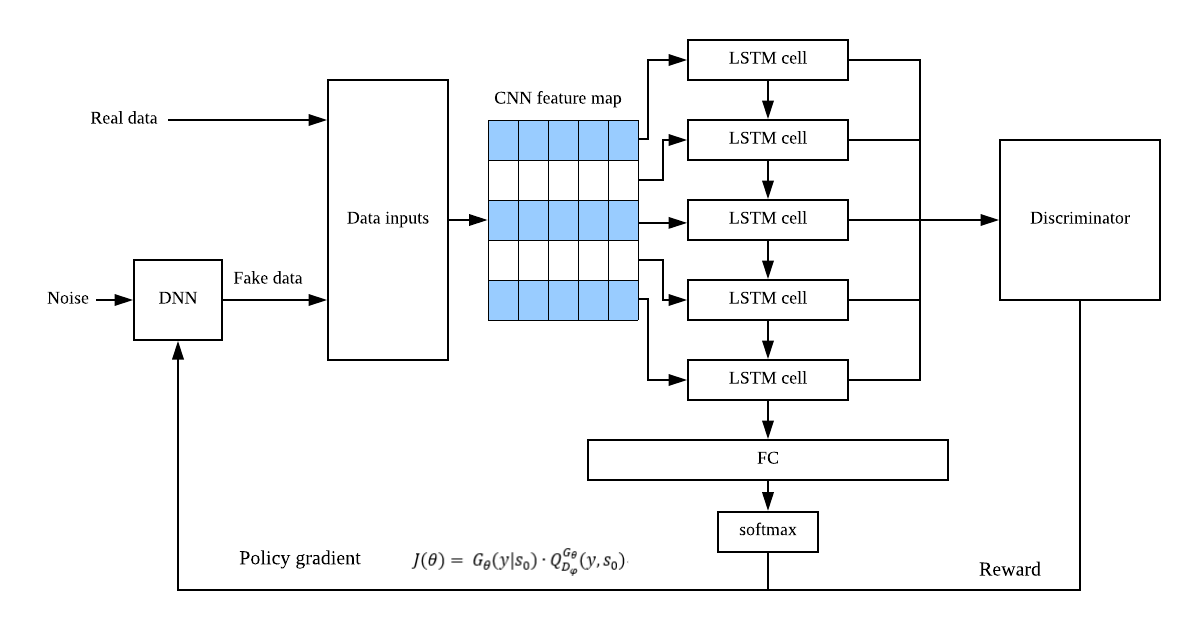
\includegraphics[width=0.9\textwidth]{gan.png}
	\end{center}
	\caption{The GAN Architecture}
	\label{RTL}
\end{figure*}

Now we can define the goal of the generator network, we have:

\begin{equation}
J(\theta) = G_\theta(y|s_0) * Q_{D_\theta}^{G_\theta}(s_0, y)
\label{eq:samplevar}
\end{equation}

The generator is supposed to generate real-like data sequence, when it takes an action, J(θ) represents the expectation value of this action’s reward. Since we generate a sequence of data at one time, we can provide a reward value for a finished sequence from discriminator, we don’t need to apply Monte Carlo Search which is used in natural language generation.
The whole process is demonstrated in Figure 3.

\subsection{Training}
We update the generator’s parameter as:

\begin{equation}
\theta = \theta + \alpha_{h} \bigtriangledown_{\theta} J(\theta)
\label{eq:samplevar}
\end{equation}

Where $\aleph_{h} \in R^{+}$ denotes the corresponding learning rate at h-th step. Also the advanced gradient algorithms such as Adam and RMSprop can be adopted here.

When updating the discriminator, there are multiple loss functions to weigh the diversity between two distributions, such as cross entropy (KL divergence), JS divergence, Wasserstein distance. W-distance performs well even on discrete distribution and ensures the training process to convergence.

\begin{equation}
W_1(\mu,\upsilon) = \inf_{\pi \in \Pi(\mu,\upsilon)} E_{(x,y) \sim \pi} [d(x,y)]
\label{eq:samplevar}
\end{equation}

Before the mid-checking, our group spent plenty of time in improving the w-distance. After going insight of the w-distance, we find any distance with Lipschitz constraint can get the similar performance of w-distance. Here is the dual from of Wasserstein distance.

\begin{equation}
\begin{split}
W_1(\mu,\upsilon) = \sup_{f} E_{x \sim \mu} [f(x)] - E_{y \sim \upsilon} [f(x)], \\
s.t. f(x) - f(y) \le d(x,y), \forall x \sim \mu, \forall y \sim \upsilon
\label{eq:samplevar}
\end{split}
\end{equation}

The second line in Equation 5 is actually Lipschitz constraint. We prove the Lipschitz constraint has guarantee on gradient directions. The Figure 4 displays the function of Lipschitz constraint.

\begin{figure}[h]
	\begin{center}
		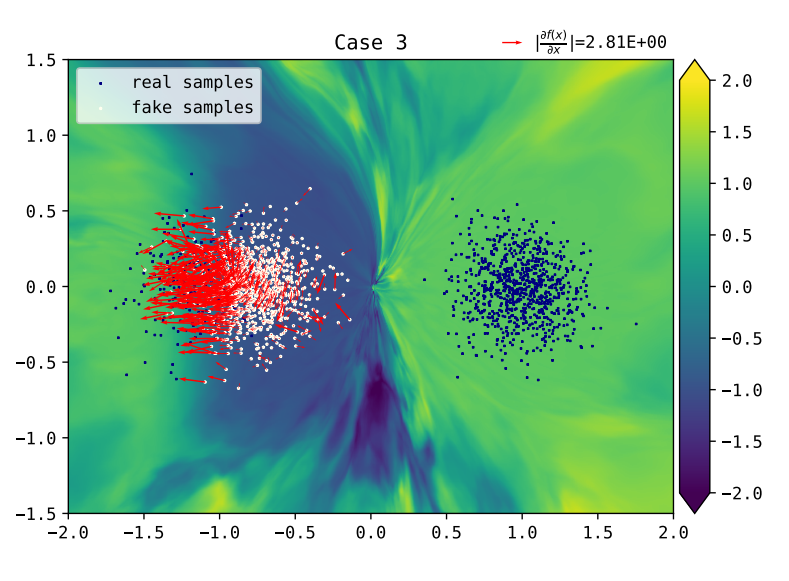
\includegraphics[width=0.45\textwidth]{lip1.png}
		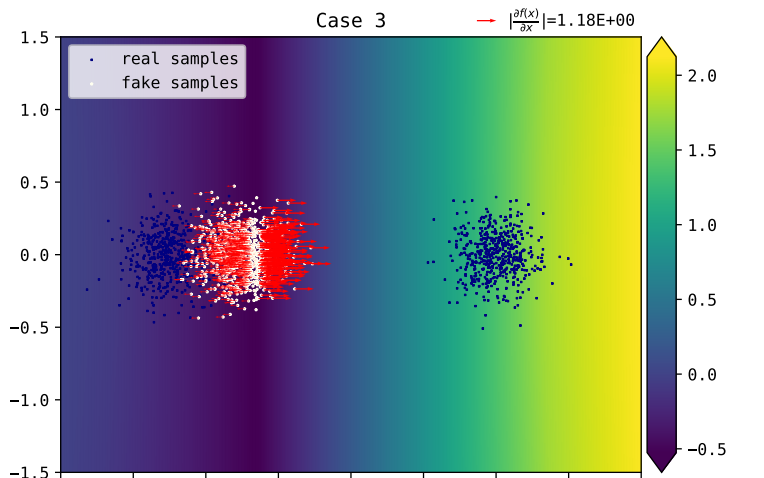
\includegraphics[width=0.45\textwidth]{lip2.png}
	\end{center}
	\caption{Above two figures illustrate the gradient direction during training process. The first one is traditional GAN using cross entropy, the second one is GAN training with Lipschitz Constraint}
	\label{RTL}
\end{figure}

So we still use the Wasserstein distance to update the discriminator. In summary, Algorithm 1 shows full details of the proposed GAN+RL for AD.

\IncMargin{1em}
\begin{algorithm}
	\SetAlgoLined
	\DontPrintSemicolon
	\LinesNumbered
	\BlankLine
	\textbf{Require:} noise-to-generated-data param $ G_{\theta} $, CLSTM param $ G_{\beta} $, discriminator param $ D_{\phi}; $ \;
	\BlankLine
   initialize the $ D_{\phi} $,$ G_{\theta}$,$ G_{\beta} $ with random weights $ \phi, \theta ,\beta$ \;
    Pre-train $ G_{\beta} $ only feeding negative real samples; \;
    \Repeat{}{
        \For{g steps}{
            Generate fake data using $ G_{\theta} $; \;
            \BlankLine
            Passing genrated data to CLSTM classifier $ G_{\beta} $, getting LSTM layers $ h_{1:T} $ and  $ G_\theta(y|s_0) $; \;
            \BlankLine
            Passing LSTM layers to discriminator, compute $Q_{D_\phi}^{G_\theta}(a = y, s = h_{1:T})$ via Eq.(1); \;
            \BlankLine
            Update generator parameter via policy gradient Eq.(3); \;
        }
        \For{d steps}{
        	Use current $ G_{\theta} $ to generate fake data; \;
        	\BlankLine
        	Passing fake date and real data to classifier $ G_{\beta} $ separately, getting LSTM layers $ h_{1:T} $; \;
        	\BlankLine
        	Passing LSTM layers to discriminator, and train discriminator $ D_{\phi} $ using Wasserstein distance. \;
        }
    }
    \BlankLine
    \caption{GAN+RL for AD network \label{IR}}
\end{algorithm}\DecMargin{1em}
 		
Firstly, we need to pre-train the C-LSTM classifier and let it to learn how to classify the normal data sequence. Noting that we don't feed positive samples, so the classifier can't classify abnormal data well, but it can classify noise-generated data well. For example, a real data sequence contains only one abnormal data, others are all normal, but this sequence is still abnormal. Comparing to generated data which comes from noise, obviously, this anomaly sequence can get higher score in pre-trained C-LSTM network. During our adversarial training procedure, we need to fix the parameters in C-LSTM network unchanged, only to update the noise-to-generated-data neural network parameters. So this method can ensure the generator to generate real-like web traffic sequence. Once the generator have learned the normal distribution, we can do anomaly assessment by evaluating the discrepancy between test data and generated data.

\subsection{Anomaly Assessment}
There are differences of our deep learning anomaly assessment method and GAN+RL anomaly assessment.

For C-LSTM classifier, it can only judge whether a sequence of data contains abnormal data, so when doing the evaluation,  we only focus on sequences in test dataset. For GAN network, the discriminator doesn't have the ability to discriminate the normal and abnormal data, and the C-LSTM classifier in generator doesn't have the ability, either. Just as introduced in 3.2, we need to design a method to compute a score which represents how large the discrepancy between learned distribution and test data. So the evaluation method in GAN doesn't focus on the sequences of test data, given a single test data, a score can be calculated, then we can judge whether this data is normal or not. The score is actually computed by the intermediate layers from the discriminator. While testing, we let the fake data and the real data both go through the discriminator, and extract the values produced by the intermediate layers in the discriminator(an intermediate layer is actually returning the latent space generated between the neural network layers). Then scores are computed by the variance between the result of the intermediate layers, which can be formulated as below:

\begin{equation}
S = (1 - \sum_{i=1}^{n}\lambda_i)L_R + \sum_{i=1}^{n}\lambda_i L_D
\end{equation}

Where $\lambda_i$ is a constant and 

\begin{equation}
L_R = \sum|x-G(z)| 
\end{equation}

\begin{equation}
L_D = \sum|f(x)-f(G(z))|
\end{equation}

$S$ is the anomaly score, $L_R$ is the residual loss, used to measure the dissimilarity between testing sample and the regenerated sample. $L_D$ is the discrimination loss, whose function is learning the feature representing. $f$ represents the intermediate layers embedded in discriminator. Multiple intermediate layers help to better evaluate the difference between the pair of discriminator’s input. 

Finally, when doing assessment, there are two criterions:
\begin{itemize}
	\item Set down a specific benchmark score, and data with score larger than this benchmark should be considered as abnormal, while the other ones are normal. However, this benchmark could only be achieved by experience, which is not a proper methods.
	\item We can guess the percentage of abnormal data in the total dataset, or this percentage can be achieved by the training dataset, and take the top percentage scores as abnormal ones. This one is more applicable, and is better for a applying to a new dataset.
\end{itemize}

These two criterions are quite the same, and we adopt the second one in our experiment due to our data preprocessing method, which will be introduced in the experiment part below.

\section{Experiments}
\subsection{Yahoo S5 Webscope Dataset and Pre-processing}
In this paper, we use the Yahoo S5 webscope dataset, which is provided as part of the Yahoo! Webscope program. It consists of four classes and we only utilize the A1 class. A1 class is based on the real production traffic to some of the Yahoo! properties, and it consists of $67$ files with a total of $94,866$ values arranged in time order, but consisting only $1669$ abnormal values, thus the data imbalance is severe. The data of the $67$ files are not continuous in time, each file has different value distribution. Fig.5 shows the first five files' data distribution. Thus we have to process each file separately, and combine them together at last.

\begin{figure}[h]
   \begin{center}
      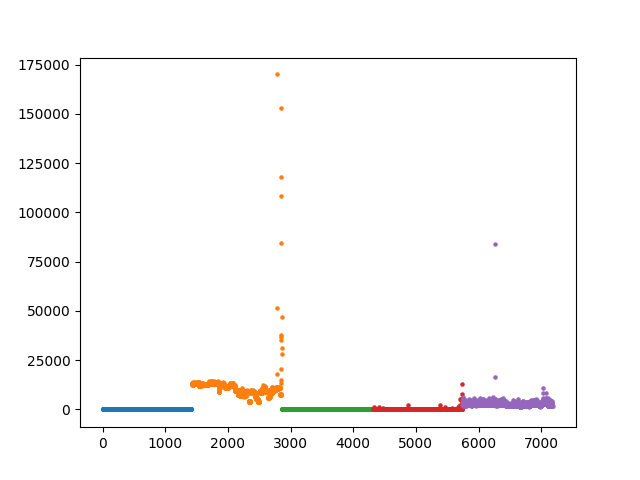
\includegraphics[width=0.45\textwidth]{value_trend.png}
   \end{center}
\caption{The values of the first 5 files, arranged in time order}
\label{RTL}
\end{figure}

We would like to make the percentage of abnormal data amount a little larger, thus a technique using the sliding window algorithm is adopted in our data preprocessing. We take a window of particular size, slide it through the sequences with a certain padding(so that its starting point can iterate through the whole file), and get data sequences of the window's size. We also shuffle the data to make the data more robust, and normalize the data into range of $(0, 1)$ using min-max scaler(as shown in Equation(9), $x^{'}$ is the normalized data). By this technique, we treat data sequences that obsess abnormal data as an abnormal sequence, and label it as abnormal.

\begin{equation}
x^{'} = \frac{x - x_{min}}{x_{max} - x_{min}}
\label{eq:samplevar}
\end{equation}

After the data preprocessing technique, a total of $90,913$ data sequences are generated and $8,556$ of them are abnormal. The percentage of abnormal data is significantly raised but still has the property of taking up a small amount. The specific parameters for the process are listed in the table below:

\begin{table}[h]
\tbl{Parameters for Sliding Window}{
\begin{tabular}{|l|l|}
	\hline
	Window Size & 60       \\ 
	\hline
	Padding Length& 1 \\
	\hline
\end{tabular}}
\end{table}

This sliding window is valid, because if a window is detected as anomalous, we only have to check the values in the window to determine the there is the abnormal sample, thus efficiency and effectiveness can be guaranteed, and using this pre-processing method, the sequence model can truly be used in anomaly detection.

\subsection{Hardware and Software Setup}
The dataset we are running on is not too large, and the models are not too time-consuming, thus an ordinary computer with Ubuntu is able to run the experiments. But for quicker results, we used a server with GeForce GTX1080 GPU to run our experiments. 


\subsection{Deep Learning Experiments}
We first constructed an LSTM+DNN model to test on the dataset and take it as one of our benchmarks. One LSTM and three layers of dense was constructed linearly. The model performed well on accuracy and precision, but dropped tremendously on recall and F1 score. The low recall is due to the fact that the model is not able to correctly categorize the abnormal data. It has a tendency to classify data into normal ones. But that's not what we wanted, we would prefer a model that has high recall scores so that abnormal data can be classified effectively.

A CNN+DNN model was also constructed, we added two dense layers linearly after the a CNN model with 6 convolutional layers, its performance was much better. This also gave us a hint, that is CNN can do very well on this dataset, spatial features do have a great impact on the detection of normal and abnormal data. 

Since adding a DNN at the last could improve the performance of the model slightly, we constructed the last deep learning model: CNN+LSTM+DNN, and reached the best result. The list for performances can be seen in the table below.

\begin{table}[h]
\tbl{Comparison of Different Model Performances}{
\begin{tabular}{|l|l|c|c|c|}
	\hline
	Model & Accuracy & Precision & Recall & F1 Score \\
	LSTM+DNN & 93.1 & 88.2 & 34.5 & 49.6 \\
	CNN+DNN & 96.7 & 95.1 & 86.5 & 90.6 \\
	CNN+LSTM+DNN & 98.6 & 96.2 & 89.7 & 92.3 \\
	\hline
\end{tabular}}
\end{table}

\subsection{GAN Experiments}
Finally, we constructed experiments on our GAN model. We use another GAN network (Houssam Zenati \cite{bibitem1}) which simply uses DNN network in generator and discriminator as benchmark. This model is designed to do anomaly detection in KDD dataset, and this data set is not time-serial, that is, neighboring data is independent with each other. So the benchmark model doesn't using the spatial and temporal information, and when updating parameters via gradients, this model is quite traditional, while our model using policy gradient. Table 4 illustrates the best performance of our model among multiple trained GAN+RL models with different hyper-parameters and the benchmark performance in Yahoo S5 Webscope Dataset. The training process was quite time-consuming, as we have to pretrain generator and train the generator and discriminator iteratively.

\begin{table}[h]
	\tbl{Performance of GAN+RL network}{
		\begin{tabular}{|l|l|c|c|c|}
			\hline
			Model & Precision & Recall & F1 Score \\
			benchmark & 85.2 & 79.7 & 82.4 \\
			Our model & \textbf{91.5} & \textbf{86.2} & \textbf{88.8} \\
			\hline
	\end{tabular}}
\end{table}

From the experiment results, we can conclude that our sequence GAN via policy gradient performs better than traditional GAN. We also find the score in Table 4 is lower than Table 3(deep learning model), because the two models'(DL and GAN+RL) evaluation methods are different, which was introduced in 3.5. Obviously, judging whether a sequence of test data contains anomaly is much easier than judging whether a single data is anomaly.

\section{Conclusion}
Though we have reached a great result on our proposed model, we still have to think about our model's pros and cons. The model is actually unstable, it is pretty hard to converge and training of it was difficult. Also, an important issue is that when we are doing loss return, the parameter updating are done by gradient descent, thus larger reward might not result in a larger gradient change. Even it does, it might contradict with action returned by the generator, with one large and one small, the model may never converge. But generally, we have achieved state-of-art result by using our GAN+RL method on dataset with both temporal and spatial features. We plan to make our model more robust and applicable on more datasets in the future.

\vfill
\vfill
\vfill
\vfill

\bibliographystyle{ieeetr}
\begin{thebibliography}{5}
	\bibitem{bibitem1} Houssam Zenati, Chuan-Sheng Foo, "Efficient GAN-Based Anomaly Detection", Workshop Track, ICLR, 2018
	\bibitem{bibitem2} Tae-Young Kim, Sung-Bae Cho, "Web traffic anomaly detection using C-LSTM neural networks", Expert Systems With Applications 106 (2018) 66–76, 2018
	\bibitem{bibitem3} Lantao Yu, Weinan Zhang, "SeqGAN: Sequence Generative Adversarial Nets with Policy Gradient", AAAI, 2017
	\bibitem{bibitem4} Bachman, P., and Precup, D., "Data generation as sequential decision making", NIPS, 3249–3257, 2015i
	\bibitem{bibitem5} Bengio, S.; Vinyals, O.; Jaitly, N.; and Shazeer,N., "Scheduled sampling for sequence prediction with recur-rent neural networks", NIPS, 1171–1179, 2015
	\bibitem{bibitem6} Chunting Zhou, Chonglin Sun, "A C-LSTM Neural Network for Text Classification", November 2015.
\end{thebibliography}
%\bibliographystyle{plain}
%\bibliography{tex}


\end{document}
% End of v2-acmtog-sample.tex (March 2012) - Gerry Murray, ACM